\documentclass{IEEEtran}

\usepackage{pslatex} % -- times instead of computer modern
\usepackage{url}
\usepackage{booktabs}
\usepackage{graphicx}
\newcommand{\code}[1]{{\small{\textsf{#1}}}}
\newcommand{\codefoot}[1]{{\textsf{#1}}}
\def\figref#1{Figure~\ref{fig:#1}}

\newcommand{\todo}[1]{{\emph{TODO: #1}}}
%\renewcommand{\todo}[1]{}

% now we have colors ;-)
\usepackage[usenames,dvipsnames]{color}
\newcommand{\tommy}[1]{{\color{red} Tommy: #1}}
\newcommand{\wolf}[1]{{\color{OliveGreen} Wolfgang: #1}}
\newcommand{\martin}[1]{{\color{blue} Martin: #1}}

\usepackage{listings}

\lstnewenvironment{Java} {\lstset{
  basicstyle=\sffamily\small,keywordstyle=\sffamily\small,xleftmargin=12pt,
  language=Java,
  columns=flexible, % add any modifications here
}}{}

\usepackage{bytefield}

%\newcommand{\obacht}[2]{\marginpar{\tiny\textbf{#1:} #2}}
\newcommand{\obacht}[2]{{\textbf{#1:} \emph{#2}}}
\renewcommand{\obacht}[2]{}

\begin{document}



\title{Patmos: a Time-predictable Dual-Issue Microprocessor\\
	{\huge Technical Report}}


%\numberofauthors{7}
%\author{
%\alignauthor
%Martin Schoeberl\\
%       \affaddr{Department of Informatics and Mathematical Modeling}\\
%       \affaddr{Technical University of Denmark}\\
%       \email{masca@imm.dtu.dk}
%% 2nd. author
%\alignauthor Pascal Schleuniger \\
%       \affaddr{DTU Informatics}\\
%       \affaddr{Technical University of Denmark}\\
%       \email{pass@imm.dtu.dk}
%% 3rd. author
%\alignauthor
%Wolfgang Puffitsch\\
%       \affaddr{Institute of Computer Engineering}\\
%       \affaddr{Vienna University of Technology}\\
%       \email{wpuffits@mail.tuwien.ac.at}
%\and  % use '\and' if you need 'another row' of author names
%% 4th. author
%\alignauthor Florian Brandner\\
%       \affaddr{INRIA}\\
%       \affaddr{COMPSYS, LIP, ENS de Lyon}\\
%       \email{florian.brandner@ens-lyon.fr}
%% 5th. author
%\alignauthor Christian W.~Probst\\
%       \affaddr{Department of Informatics and Mathematical Modeling}\\
%       \affaddr{Technical University of Denmark}\\
%       \email{probst@imm.dtu.dk}
%% 6th. author
%\alignauthor Sven Karlsson\\
%       \affaddr{DTU Informatics}\\
%       \affaddr{Technical University of Denmark}\\
%       \email{ska@imm.dtu.dk}
%\alignauthor Tommy Thorn\\
%       \affaddr{Unaffiliated Research}\\
%       \affaddr{California, USA}\\
%       \email{tommy@thorn.ws}
%}
%





\maketitle
%\thispagestyle{empty}

\begin{abstract}
This TR shall evolve to the documentation of Patmos. In the mean time it is intended to collect design notes and discussions.

\end{abstract}



\section{Introduction}

Real-time systems need a time-predictable execution platform so that the worst-case execution time (WCET) can be statically estimated. It has been argued that we have to rethink computer architecture for real-time systems instead of trying to catch up with new processors in the WCET analysis tools~\cite{tpca:jes, pret:dac2007}.

We present the time-predictable processor Patmos as one approach to attack the complexity issue of WCET analysis. Patmos is a static scheduled, dual-issue RISC processor that is optimized for real-time systems.



%\section{Related Work}
%\label{sec:related}


\section{The Architecture of Patmos}
\label{sec:arch}

\subsection{Pipeline}

Figure~\ref{fig:pipeline} shows an overview of Patmos' pipeline.

\begin{figure*}[t]
    \centering
    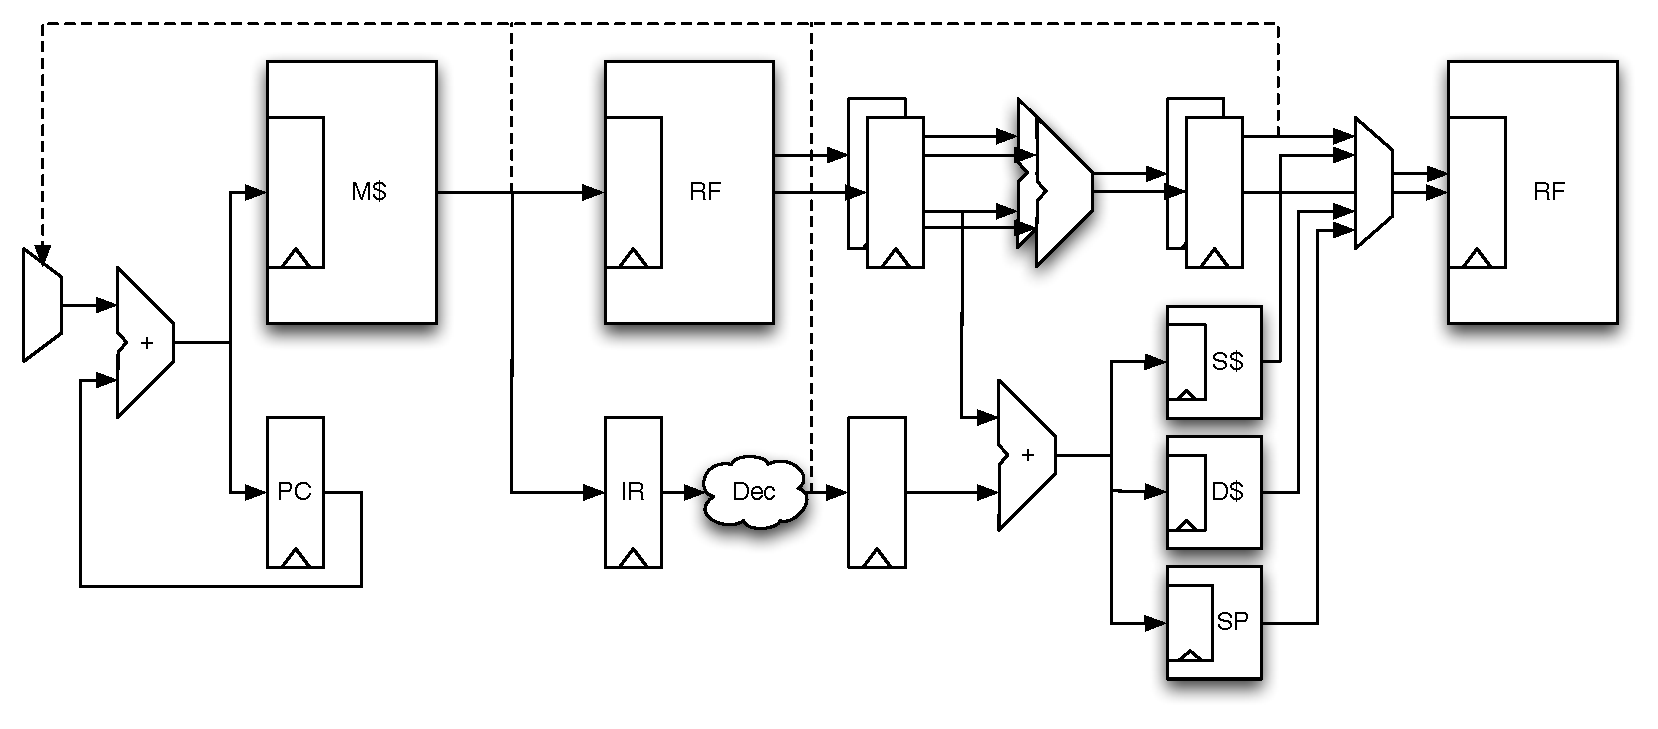
\includegraphics[scale=0.6]{fig/pipeline}
    \caption{Pipeline of Patmos with fetch, decode, execute, and memory/write back stages.}\label{fig:pipeline}
\end{figure*}

\subsection{Instruction List}

Bit 31 indicates the length of the instruction. If it is 1, a second word can be executed in the second pipeline.

\begin{itemize}

\item ALU immediate (add, or, and, xor), the function is indicated with \emph{ff}: \\

\begin{bytefield}{32}
\bitheader[b]{0-31}\\
\bitbox{1}{x} & \bitbox{3}{000} & \bitbox{2}{ff} &
\bitbox{4}{Pred} & \bitbox{5}{Rd} & \bitbox{5}{Rs1} &
\bitbox{12}{Constant}\end{bytefield}\\

\item ALU immediate long (uses second slot for the 32-bit constant and
  thus is allowed only in the first slot): \\

\begin{bytefield}{32}
\bitheader[b]{0-31}\\
\bitbox{1}{1} & \bitbox{5}{00100} &
\bitbox{4}{Pred} & \bitbox{5}{Rd} & \bitbox{5}{Rs1} & \bitbox{5}{} &
\bitbox{7}{Function}\end{bytefield}\\

\item ALU function: \\

\begin{bytefield}{32}
\bitheader[b]{0-31}\\
\bitbox{1}{x} & \bitbox{5}{00101} &
\bitbox{4}{Pred} & \bitbox{5}{Rd} & \bitbox{5}{Rs1} & \bitbox{5}{Rs2} &
\bitbox{7}{Function}\end{bytefield}\\

\item Branch relative (use predicates): \\

\begin{bytefield}{32}
\bitheader[b]{0-31}\\
\bitbox{1}{x} & \bitbox{5}{00110} &
\bitbox{4}{Pred} &
\bitbox{22}{Offset}\end{bytefield}\\

\item Load 16-bit constant (low sign extend, high): \\

\begin{bytefield}{32}
\bitheader[b]{0-31}\\
\bitbox{1}{x} & \bitbox{5}{00111} &
\bitbox{4}{Pred} & \bitbox{5}{Rd} & \bitbox{1}{d} &
\bitbox{16}{Constant}\end{bytefield}\\

\item Compare (constant could be Rs2 field). It is predicated and has a
destination predicate field: \\

\begin{bytefield}{32}
\bitheader[b]{0-31}\\
\bitbox{1}{x} & \bitbox{5}{01000} &
\bitbox{4}{Pred} & \bitbox{5}{Pdest} & \bitbox{5}{Rs1} & \bitbox{5}{Rs2} &
\bitbox{7}{Function}\end{bytefield}\\


\item Load with a memory type (direct main memory will be a split instruction). Offset counts in natural word lenght, e.g. 4 bytes for a word: \\

\begin{bytefield}{32}
\bitheader[b]{0-31}\\
\bitbox{1}{x} & \bitbox{5}{01001} &
\bitbox{4}{Pred} & \bitbox{5}{Rd} & \bitbox{5}{Ra} &
\bitbox{5}{Type} & \bitbox{7}{Offset}\end{bytefield}\\

\item Store with a memory type (direct main memory will be a split instruction): \\

\begin{bytefield}{32}
\bitheader[b]{0-31}\\
\bitbox{1}{x} & \bitbox{5}{01010} &
\bitbox{4}{Pred} & \bitbox{5}{Type} & \bitbox{5}{Ra} & \bitbox{5}{Rs} &
\bitbox{7}{Offset} \end{bytefield}\\


%\item xxx: \\
%
%\begin{bytefield}{32}
%\bitheader[b]{0-31}\\
%\bitbox{1}{x} & \bitbox{5}{00---} &
%\bitbox{4}{Pred} & \bitbox{5}{Rd} & \bitbox{5}{Rs1} & \bitbox{5}{Rs2} &
%\bitbox{7}{Function}%\end{bytefield}\\

\end{itemize}

Some more instructions to be defined: start multiplication, load result (from multiplication and external memory load), wait on memory, branch and link, load method cache, load and store predicates, store multiplication result, interrupt handling -- we will support multithreading, therefore the full processor context needs to be save- and restorable,...

\martin{Do we need exceptions? The only two I can think of are null pointer and divide by zero. Is it worth implementing (exact) exceptions for this or do we just leave it to the compiler?}

\wolf{I do not think that we need exceptions besides null pointer and division by zero (and even those could be raised explicitly). But we have to think about the handling of interrupts: What do we do if we get an interrupt between issuing a memory load or the start of a multiplication and retrieving the result? Disable interrupts in between? Make result registers writable so we can restore the original state?}

\wolf{We also need to think about the handling of exceptions on the higher-language level. Can we support Java-style exceptions efficiently?}

\todo{The above should be generated from a common definition of the ISA (which is used by all parts of the project).}

\section{Discussion}


\tommy{Martin (jokingly?) told me that Patmos aims to
beat YARI. I'm all for it as I've been trying to do the same for a long
time. However I've found it very difficult to beat a simple single-
issue RISC. Although I think I have the answer, it's a very
different path from Patmos and I'll not push it here.}

\martin{Partially a joke, partially I really would like to beat it ;-)
Serious, Patmos will be optimized for WCET and not average
case performance. On the other side it should no be too slow.}

\tommy{In YARI, fMAX (AKA 1/cycle-time) is strongly correlated to the
 width of the widest mux in any stage. Another way to say this,
 the more things a register depends on, the slower it gets.}
 
\martin{Yes, I'm a little bit afraid of the forwarding muxes from the
two pipelines. We have not yet implemented that part.

I know that Sven wants to pipeline the forwarding. This
costs one cycle latency and we don't know if this can be
compensated by clever instruction scheduling in the
compiler.}

\wolf{In my hobby design I use registers that do nothing but feed the
forwarding. This lets the synthesis place the registers freely and
makes forwarding less painful by reducing the interconnect delay. Of
course, if the synthesis is clever, it can duplicate registers to
achieve the same thing, but doing it explicitly helped at least in my
design.}

\tommy{Ways to improve this in order of effectiveness:

 1) Change the ISA

 2) Whenever possible, share sources for a register, fx. to copy a
    value consider adding it to zero rather than having a separate
    mux input, and, failing everything else,

 3) move logic up to an earlier stage (unfortunately this usually
    implies increasing latencies).}

 \tommy{A consequence of this fact was to not use interlocking in the
 pipeline at all, but to restart the pipeline whenever a hazard
 was violated. This way there's only one source for the
 instruction for every stage in the pipeline (along with a valid
 bit which is cleared by restart and checked only by logic that
 would commit state).}

\martin{We also plan to not use interlocking, but no pipeline restarting.
All instructions (except one) do not stall at all. (This is similar
to the JOP pipeline).}

\tommy{Replace my use of interlocking with stalling. The ability to
  stall the pipeline is expensive. Restarting the pipeline (and
  replaying the original instruction) achieves the same effect with
  less cycle-time impact at the cost of potentially higher resume
  latency compared to true stalling. (Powerwise, stalling is better).}
  
\martin{The intention of Patmos is to have no stalls at all -- with one
exception. So no stalling, no restart. The single exception is main
memory access. In that case we use a split load and an explicit wait
for the result. That wait is somehow \emph{pipeline stalling}. Perhaps
we do it the JOP way and fill the pipeline with wait instructions that
do nothing and only one stage needs to check the memory ready.
BTW: this is also the reason for the ready counter in SimpCon we
discussed some long time ago. It is used to restart the pipeline a 
few cycles earlier so the load instruction is in EX stage when the actual
data arrives.}

 \tommy{One very real example I struggled with load latency. MIPS
 defines a one-cycle load latency. Violating this in YARI would
 cause a pipeline restart, originally a five cycle penalty.
 Unfortunately, the JIT we were using (CACAO) has a pretty
 naive code generator and even making it emit a nop for the
 load was non-trivial.}

 \martin{We have more freedom with the VLIW approach to
 expose latencies and the compiler should be smart ;-)}

\tommy{I tried quite a lot of alternatives:
 0. simply completing the load in one cycle (really hurt fMAX)
 1. moving the EX stage down to the 2nd half of the load (now
    the hazard is on loads whose address register isn't ready
    two cycles ahead of the load),
 2. A hybrid, where only 8- and 16-bit loads suffer the additional
   latency.}

\tommy{ Without measurements I couldn't predict which would win, but
 real-life results were counter-intuitive and in the end I got the
 best result with

 3. keeping it was, but reducing the hazard penalty to two
  cycles (IIRC).}

\tommy{After much mux optimization
  (cf.~http://portal.acm.org/citation.cfm?id=968291 and
  http://portal.acm.org/citation.cfm?id=1065692)
 the bypass network and register file ended up being the critical
 path and the only way to I know to improve that would be at
 the cost of more hazards (eg.~restart on unsupported forwards).}


\tommy{How does this apply to Patmos?
* Unlike YARI, Patmos doesn't implement an existing ISA, so to
 me an architectural simulator is even more critical. Developing
 the compiler against an evolving SystemC implementation
 seems somewhat wanting.}

\tommy{* Many design decision in the paper strikes me as somewhat
 premature in the absence of measurements, but I guess I
 shouldn't worry about that.}

\martin{You're right. However, we even would need WCET analysis instead
of measurements to judge the decisions. Even harder to do at this
stage. So we can only perform educated guesses.}

\tommy{* Assuming (optimistically) that the compiler can extract an avg. IPC
 of 1.6, Patmos would need an fMAX of 56 MHz just to be at parity
 with YARI and that's not accounting for the overhead of the two-
 instruction loads. I'm concerned that the bypass network may not
 be able to go that fast.}

\martin{Something to be evaluated....}


\subsection{More on load/store}

\tommy{Sign extended loads hurts FPGA implementations much more than real
silicon because muxes are very expensive here. I strongly recommend
making all loads zero extending and provide explicit sext8 and sext16
instructions. (This matches the RISC philosopy of exposing the real
cost of operations).

(Caution: The Alpha route of providing only word-level accesses proved to be a mistake (IO
problems and more) and they had to provide byte and short level accesses
in the second version of the architecture.)}

\tommy{
Load and store offset of 7 bits is too small. Assuming it's signed
(right?) that's just [-64; 63]. Even if scaled by four for word
accesses that's still just [-256; 248]. Luckily, there are bits that can
be recovered}

\martin{to be explored}

\tommy{ Merge "ALU function" and "Compare" -> save one bit

- Load/Store to use natual scaling of offset.

 It's very rare in practice for the offset not to be naturally
 aligned, so we can save some redundant bits at the cost of more
 muxing in the address computation.}
 
 \martin{agree on both, although compare has an additional field for
 the predicate destination.}




\section{Conclusion}
\label{sec:conclusion}

Patmos is the next cool thing in the dry world of real-time systems.



\section*{Source Access}

When will we be able to open the git for the public?

\bibliographystyle{abbrv}
\bibliography{other,msbib}


\appendix

\section{Notes}

\begin{itemize}
\item Explore time-predictable ideas
\item Platform for the EC funding proposal, CMP experiments, NoC,...
\begin{itemize}
\item Method \$, stack \$, SMP (w. pointer remapping?)
\item \emph{typed} load store instructions
\end{itemize}
\item MIPS style ISA, 2 ALUs, 1 LS unit
\item Predicates, also for branches
\item Double clock the RF $=>$ 4 read and 2 write ports
\item Variable length instructions (32/64 bit) -- dual M \$ idea
\item Explicit instructions for call, M\$ load, SPM load/store
\item no stalls -- use explicit wait for external memory operations
\item 1st slot is general, 2nd slot \emph{just} ALU operations
\end{itemize}

\subsection{Getting Started}

\begin{itemize}
\item A paper on the concept
\begin{itemize}
\item Core components (RF, ALU, Fetch) in VHDL
\item SystemC simulation
\item Assembler + ISA simulator in Java
\end{itemize}
\item FPGA implementation
\item C/C++ compiler
\item Explore SPM, M\$, S\$ w. a compiler
\item RT-Java? (JamaicaVM or Fiji)
\item Part of the EC funding proposal
\item Talk with Edward and Isaac
\end{itemize}

\subsection{Instruction Set}

\begin{itemize}
\item 1 bit length, 32 register, 8 predicates
\item ALU immediate is most constraining $=>$ 2 forms
\begin{itemize}
\item short constant: 12 bit sign extending, perhaps only 4 functions: add, or, and, xor
\item long constant: use 2nd instruction slot for a 32 bit constant
\end{itemize}
\item ALU, shift, shift constant
\item Branch relative (uses predicate)
\item load 16 bit constant (low sign extending, high)
\item load/store register indirect + offset, typed
\item branch and link
\item \emph{special} instructions
\begin{itemize}
\item start multiplication, load result
\item wait on memory operation (split load)
\item load method cache
\item calculation w. predicates (spill/fill)
\begin{itemize}
\item or map P to R31?
\item wide or/and
\end{itemize}
\item parallel load (both slots) from S\$
\end{itemize}
\end{itemize}

\subsection{Tasks}

\begin{itemize}
\item Some VHDL/FPGA experiments (MS, PS)
\item SystemC prototype (MS)
\item Assembler
\item Compiler backend
\item Simulator
\end{itemize}


\subsection{LLVM}

Thanks to Wolfgang a first LLVM port is available! Here are the instructions to build and use it:

\begin{Java}
./configure --target=patmos
make
llvm-gcc -emit-llvm -o foo.bc -c foo.c
./Release/bin/llc -march=patmos foo.bc
\end{Java}

\wolf{I will rework the instruction selection as soon as we have a
  sufficiently detailed ISA. Unless we create some \emph{very} strange
  instructions, this should not be a major issue.

Do not hesitate if I you feel like looking into the instruction
scheduling/bundling. I will work on it eventually, but it might take a
while.}

\subsection{Memory Accesses}

\wolf{There are (at least) two ways to split memory loads. Explicit wait and
load: \texttt{ldm addr; wait; dest = ldx \$mem}, or implicit wait:
\texttt{ldm addr; dest = ldx \$mem}. Depending on the available units,
the former may allow pipelined memory accesses:

\medskip
\begin{tabular}{ll}
  Pipeline A & Pipeline B \\
  \hline
  \texttt{ldm addrA} & \\
  \texttt{wait for rdycnt<=1} & \texttt{ldm addrB} \\
  \texttt{destA = ldx \$mem} & \\
  \texttt{ldm addrC} & \texttt{wait for rdycnt<=1} \\
                     & \texttt{destB = ldx \$mem} \\
  \texttt{wait for rdycnt<=1} & \\
  \texttt{destC = ldx \$mem} & \\
\end{tabular}

\medskip
Also, the \texttt{ldx} part of the loads can go through the ALU, which
\emph{might} reduce multiplexing in the forwarding logic (only the
ALUs ever produce results). The \texttt{wait} could maybe be omitted
for stack and scratchpad memory accesses.

On the other hand, implicit waiting clearly wins in terms of code size
and instructions to be executed (more free slots for other stuff).  I
think that implicit waiting is more profitable for Patmos, but
educated guesses (or facts\ldots) would be very welcome.}

\martin{I would argue that split loads are only for the main memory and
caches that \emph{might} miss. Access to stack cache and SPM should
be a guaranteed hit. BTW: normal memory loads can only be scheduled
in the first instruction slot -- we have only one l/s unit. However, Florian
convinced me that double ld/st to the stack can be beneficial for register
spill and fill. So the plan is to allow stack ld/st (we just need word here....)
in both slots.}

\wolf{Fast access to the stack is a good idea, the following only
  applies to ``normal'' memory accesses. Loading the results of all
  loads via the ALUs would be a cheap way to free the first slot for
  issuing loads/stores and jumps. There is no real need to put that
  into the memory unit (is there?). Do you assume that waiting is
  handled in the l/s unit? In my opinion, a separate stall unit that
  is accessible from both pipelines would be nice (forwarding does not
  get more complicated). With implicit waiting, three consecutive
  accesses could look like this:

  \medskip
  \begin{tabular}{ll}
    Pipeline A & Pipeline B \\
    \hline
    \texttt{ldm addrA} & \\
    \texttt{ldm addrB} & \texttt{destA = ldx \$mem} \\
    \texttt{ldm addrC} & \texttt{destB = ldx \$mem} \\
                       & \texttt{destC = ldx \$mem} \\
  \end{tabular}
}

\end{document}
